%%%%%%%%%%%%%%%%%%%% author.tex %%%%%%%%%%%%%%%%%%%%%%%%%%%%%%%%%%%
%
% sample root file for your "contribution" to a proceedings volume
%
% Use this file as a template for your own input.
%
%%%%%%%%%%%%%%%% Springer %%%%%%%%%%%%%%%%%%%%%%%%%%%%%%%%%%


\documentclass{svproc}
\usepackage{marvosym}
%
% RECOMMENDED %%%%%%%%%%%%%%%%%%%%%%%%%%%%%%%%%%%%%%%%%%%%%%%%%%%
%
\usepackage{graphicx}

% to typeset URLs, URIs, and DOIs
\usepackage{url}
\usepackage{hyperref}
\usepackage[english, russian]{babel} 
\usepackage{amsmath} 
\def\UrlFont{\rmfamily}
\providecommand{\doi}[1]{doi:\discretionary{}{}{}#1}

\def\orcidID#1{\unskip$^{[#1]}$}
\def\letter{$^{\textrm{(\Letter)}}$}

\begin{document}
\mainmatter              % start of a contribution
%
\title{Об использовании деревьев решений для идентификации локальных экстремумов в параллельном алгоритме глобальной оптимизации}
%
\titlerunning{Global Optimization ...}  % abbreviated title (for running head)
%                                     also used for the TOC unless
%                                     \toctitle is used
%
\author{K.~A.~Barkalov\inst{1}\letter\orcidID{0000-0001-5273-2471} \and I.~G.~Lebedev\inst{1}\letter\orcidID{0000-0002-8736-0652} \and D.~I.~Silenko\inst{1}\letter\orcidID{0000-0002-2578-9699}}
%
\authorrunning{K.~A.~Barkalov et al.} % abbreviated author list (for running head)
%
%%%% list of authors for the TOC (use if author list has to be modified)
\tocauthor{K.~A.~Barkalov and I.~G.~Lebedev, and D.~I.~Silenko}
%
\institute{Lobachevsky State University of Nizhny Novgorod, Nizhny Novgorod, Russia \\
\email{konstantin.barkalov@itmm.unn.ru, ilya.lebedev@itmm.unn.ru, rotor12587@mail.ru}
}

\maketitle              % typeset the title of the contribution

\begin{abstract}
В работе рассматривается решение задач многомерной глобальной оптимизации с применением decision tree для выявления областей притяжения локальных минимумов. Целевая функция задачи задана как ''черный ящик''. 
Мы лишь предполагаем, что она удовлетворяет условию Липшица с неизвестной константой. 
Для поиска глобального минимума в задачах такого типа используется алгоритм глобального поиска.
В настоящей работе мы предлагаем способ выделения окрестностей локальных экстремумов целевой функции на основе анализа накопленной поисковой информации.
Проведение такого анализа средствами машинного обучения позволяет принять решение о запуске локального метода, который может ускорить сходимость алгоритма. Выдвинутое предположение подтверждается результатами вычислительных экспериментов, демонстрирующих ускорение при решении серии тестовых задач. 
% We would like to encourage you to list your keywords within
% the abstract section using the \keywords{...} command.
\keywords{Global optimization $\cdot$ Multiextremal functions $\cdot$ Parallel computing $\cdot$  Decision tree}
\end{abstract}
%

\section{Введение}

В работе рассматриваются параллельные алгоритмы для решения задач многомерной глобальной оптимизации. Такие задачи часто возникают в случае, когда требуется выбрать значения параметров исследуемой математической модели, при которых результаты моделирования наилучшим образом соответствуют экспериментальным данным.
Для решения задач указанного класса известен широкий спектр алгоритмов, он основанных на идее случайного поиска \cite{fio_bib1, fio_bib2, fio_bib3} метаэвристических алгоритмов, до детерминированных алгоритмов, гарантирующих сходимость к глобальному минимуму \cite{fio_bib4, fio_bib5, fio_bib6}. 
Поскольку в реальных задачах глобальной оптимизации каждое вычисление значения функции (называемое в дальнейшем trial) представляет собой весьма трудоемкую операцию, необходимо уменьшить количество таких trials. Этого можно добиться целенаправленным выбором вариантов в процессе поиска оптимального решения, отсекая бесперспективные подобласти поиска и исследуя только те, в которых может содержаться решение задачи. На этой идее основывается global search algorithm (GSA) \cite{fio_bib7}. В данной работе мы попробуем объединить GSA и метод локальной оптимизации (Hooke--Jeeves method) с целью уменьшить количество проводимых испытаний. При этом принятие решения о запуске локального метода будет осуществляться с помощью decision tree.

Алгоритмы локальной оптимизации предназначены для определения лишь одного из локальных экстремумов на множестве допустимых решений, в котором целевая функция принимает экстремальное (максимальное или минимальное) значение. 
Среди локальных методов традиционно выделяют методы нулевого порядка и градиентные методы  (1-го и 2-го порядков) \cite{fio_bib8,fio_bib9}.
Отметим, что применение методов первого порядка (не говоря уже о втором) в задачах с функциями вида ''черный ящик'' затруднено, т.к. здесь возникает проблема численной оценки градиента. Поэтому мы будем рассматривать в дальнейшем только методы нулевого порядка.

Для того, чтобы понять, в какой момент лучше всего запускать локальный метод в рамках глобального поиска, мы будем использовать алгоритм на основе decision tree.
На первой стадии поиска происходит накоплении поисковой информации в виде результатов проведенных испытаний.
Результаты испытаний мы используем для тренировки decision tree, что позволяет получить кусочно-линейную аппроксимацию целевой функции и  предсказывать на ее основе поведение целевой функции. Для этого бы будем сравнивать значения функции в точках, соседних к той, которую считаем подозрительной на локальный минимум. И на основе кусочной-линейной аппроксимации принимать решение, находится очередная точка испытания в области притяжения локального минимума или нет.

Основная часть статьи имеет следующую структуру. 
В Section \ref{SecPS} рассмотрена постановка задачи глобальной оптимизации, сделаны основные предположения о целевой функции .
В Section \ref{SecA} приведено описание используемых методов и подходов.
В частности, в Section \ref{SecGSA} обсуждается основная идея global search algorithm, приведены его вычислителные правила.
Section \ref{SecHG} содержит описание используемого метода локального поиска.
Способ построения аппроксимаций функции с использованием деревьев решений описан в Section \ref{SecDT}.
Новый алгоритм, объединяющий глобальный и локальный поиск на основе использования деревьев решений, приведен в Section \ref{SecGSAL}.
В следующем разделе обсуждаются особенности асинхронной схемы распараллеливания нового алгоритма.
Section \ref{SecR} содержит результаты экспериментов, проведенных на параллельной вычислительной системе с distributed memory.
В Заключении представлены основные выводы по проделанной работе.

\
\section{Problem statement}\label{SecPS}

Рассмотрим задачу поиска глобального минимума функции $\varphi(y)$ в гиперинтервале $D=\{ y\in\ R^N:\ a_i\le\ y_i\le\ b_i,\ 1\le\ i\le\ n \}$. При этом будем предполагать, что функция удовлетворяет the Lipschitz condition с априори неизвестной константой $L$, что соответствует ограниченности изменения значений функции при ограниченной вариации аргумента. Это предположение можно интерпретировать (применительно к прикладным задачам) как отражение ограниченности мощностей, порождающих изменения в моделируемой системе. 




\begin{equation} \label{sec:problem}   
\varphi(y^*) = min\{\varphi(y):y\in D\}, D = \{y \in R^N : a_i \leq y_i \leq b_i, 1 \leq i \leq N \},
\end{equation}
где $a,b \in R$ есть заданные векторы.


\begin{displaymath}
|\varphi(y_1)-\varphi(y_2)|\leq L\parallel y_1-y_2 \parallel
,y_1,y_2 \in D, 0<L< \infty.
\end{displaymath}




Численное решение задачи (\ref{sec:problem})   сводится к построению оценки $ y_k^\ast\in\ D$ , отвечающей некоторому понятию близости к точке $y^\ast$ (например, ${||y^\ast-y}_k^\ast||\le\ \varepsilon$, где $\varepsilon\geq0$ есть заданная точность) на основе конечного числа $k$ вычислений значений целевой функции. Относительно класса рассматриваемых задач предполагается, что оптимизируемая функция $\varphi(y)$ может быть задана алгоритмически, как результат работы некоторой подпрограммы или библиотеки.

Задачи многоэкстремальной оптимизации имеют существенно более высокую трудоемкость решения по сравнению с другими типами оптимизационных задач, т.к. глобальный оптимум является интегральной характеристикой решаемой задачи и требует исследования всей области поиска. Как результат, поиск глобального оптимума сводится к построению некоторого покрытия (сетки) в области параметров, и выборе наилучшего значения функции на данной сетке. При использовании равномерных сеток вычислительные затраты на решение задачи растут экспоненциально с ростом размерности.

\section{Используемые алгоритмы}\label{SecA}

Основная идея подхода к построению более экономной неравномерной сетки заключается в том, что ее точки вычисляются последовательно, а целевая функция рассматривается как реализация некоторого случайного процесса. Решающие правила алгоритма построения сетки конструируются таким образом, что очередная точка сетки соответствует точке глобального минимума математического ожидания значений функции. Эта точка записывается в список известных значений и итерации повторяются. Так происходит до тех пор, пока не достигнут один из выбранных критериев остановки: расстояние между точками проведенных испытаний становится меньше заданного значения или же достигается установленное максимальное число итераций. \cite{fio_bib10}

При решении многомерных задач применяется редукция размерности (т.е. сведение многомерной задачи к эквивалентной одномерной) с использованием кривых Пеано. Они позволяют свести многомерную задачу минимизации в области $D$  к одномерной задаче минимизации на отрезке $[0, 1]$

\begin{displaymath}
\varphi(y(x^\ast))\ =\ min\{\varphi(y(x)):\ x\epsilon[0,\ 1]\}
\end{displaymath}

где функция $\varphi(y(x^\ast))$  удовлетворяют более общему H{\"o}lder condition

\begin{displaymath}
\left|\varphi (y \left(x_1\right))- \varphi (y \left(x_2\right)\right )|\le\ H\left|x_1-x_2\right|^\frac{1}{N},\ x_1,\ x_2\epsilon[0,1].
\end{displaymath}

Поэтому вместо исходной задачи минимизации функции $\varphi(y)$ в области $D$ можно рассматривать минимизацию одномерной функции $f(x)\ =\ \varphi(y(x))$, удовлетворяющей the H{\"o}lder condition, при $ x\in [0,1]$.

\subsection{Многомерный параллельный алгоритм глобального поиска}\label{SecGSA}

Основные шаги parallel global search algorithm состоят в следующем.

На подготовительном шаге параллельно проводятся $p$ trials в произвольных внутренних точках $x^1, ...,x^p$ отрезка $[0,1]$, что соответствует первой итерации  алгоритма. 

Если выполнено $n \geq 1$ итераций, которым соответствуют $k=k(n)$ проведенных испытаний в точках $x^i, 1\leq i\leq k$, то точки $x^{k+1},\ldots,x^{k+p}$ поисковых испытаний следующей $(n+1)$-й итерации будут вычисляться в результате выполнения следующих действий.

\begin{enumerate}

\item  Переупорядочить (нижним индексом) точки $x^i, 1\leq i\leq k$, а также граничные точки отрезка [0,1] в порядке возрастания координаты:
 \begin{equation}
\label{agp1_sort}
	0=x_0<\ x_1<\ ...\ <x_{k+1}=1.
	\end{equation}
	и сопоставить им значения $z_i=f(x_i)$. 
	
\item  Вычислить текущие нижние оценки $M$ неизвестной H{\"o}lder constani $H$:
 \begin{equation}
\label{agp2_mu}
	\mu=max\left\{\frac{|z_i-z_{i-1}|}{{{(x}_i-x_{i-1})}^{1/N}},\ i=1,\ldots,k\right\},\ M=\ \left\{\begin{matrix}r\mu,\ \mu>0,\\1,\ \mu=0,\\\end{matrix}\right.\
	\end{equation}
где $r>1$ есть параметр алгоритма. Данный параметр регулирует надежность алгоритма: большие значения $r$ обеспечивают гарантированное нахождение глобального минимума, выбор меньшего значения --- ускоряет сходимость алгоритма
   
\item  Для каждого интервала $(x_{i-1},x_i), 1\leq i\leq k+1,$ вычислить величину $R(i)$, называемую \textit{характеристикой} интервала, в соответствии с формулами

\begin{equation}
\label{agp3_R1}
R(1)=2\Delta_1-4\dfrac{z_1}{M}, \; R(k+1)=2\Delta_{k+1}-4\dfrac{z_k}{M},
\end{equation}

\begin{equation}
\label{agp3_Ri}
R(i)=\Delta_i+\dfrac{(z_i-z_{i-1})^2}{M^2\Delta_i}-2\dfrac{z_i+z_{i-1}}{M},1<i<k+1,
\end{equation}
где \(\Delta_i=(x_i-x_{i-1})^\frac{1}{N}\).
   
\item   Упорядочить характеристики $R\left(i\right),\ 1\leq i \leq k+1,$ в порядке невозрастания 
\begin{equation}
\label{agp4_R_sort}
	R\left(t_1\right)\geq\ R\left(t_2\right)\geq...\geq\ R\left(t_k\right)\geq\ R(t_{k+1}),\ 
\end{equation}	
и выбрать $p$ интервалов с номерами $t_j,\ 1\le\ j\le\ p$, с наибольшими значениями характеристик.

\item В выбранных интервалах вычислить точки $x^{k+j},\ 1\leq j\leq p,$ в соответствии с формулами
\begin{equation}
\label{agp5_x1}
	x^{k+j}=\frac{x_{t_j}+x_{t_j-1}}{2},\ t_j=1,\ t_j=k+1,
\end{equation}	
	\begin{equation}
\label{agp4_xi}	
	x^{k+1}=\frac{x_{t_j}+x_{t_j-1}}{2}-sign\left(z_{t_j}-z_{t_j-1}\right)\frac{1}{2r}\left[\frac{\left|z_{t_j}-z_{t_j-1}\right|}{\mu}\right]^N,\ 1<t_j<k+1.
\end{equation}	

\end{enumerate}

Очередные $p$ испытаний проводятся параллельно, в вычисленных по формулам (\ref{agp5_x1}), (\ref{agp4_xi}) точках $x^{k+j},\ 1\leq j\leq p$. После проведения испытаний их результаты заносятся в информационную базу, и алгоритм переходит к расчету новых точек испытаний.

Отметим, что в прикладных оптимизационных задачах процесс проведения trial является, как правило, значительно более трудоемким по сравнению с расчетом точки испытания.

Алгоритм останавливает свою работу в случае, если хотя бы для одного значения $t_j,\ 1\le\ j\le\ p$ из (\ref{agp4_R_sort}) выполняется условие \(\Delta_{t_j} < \varepsilon\). Данный критерий остановки (наряду с обычным для итерационных методов критерием, ограничивающим число выполненных итераций) используется в прикладных задачах оптимизации, в которых точка глобального минимума $x^*$ заранее неизвестна. 
	 
При решении тестовых задач, в которых точка глобального минимума $x^*$ является  известной, можно использовать также и критерий остановки по попаданию в окрестность глобального минимума. В этом случае метод прекращает работу, если хотя бы для одного значения $t_j,\ 1\le\ j\le\ p$ из (\ref{agp4_R_sort}) выполняется условие $\left|x_{t_j}-\ x^\ast\right| < \varepsilon.$
	
В качестве итоговой оценки глобально-оптимального решения рассматриваемой задачи выбираются значения 
\begin{equation}
f_k^*=\min_{1\leq i \leq k}f(x_i), \; x_k^*=arg \min_{1\leq i \leq k}f(x_i).
\end{equation}



Обоснование данного способа организации вычислений см. в \cite{fio_bib20}. Модификации, учитывающие наличие ограничений-неравенств в задаче, а также информация о производной целевой функции, представлены в \cite{fio_bib12, fio_bib9, fio_bib11}.


\subsection{Hooke--Jeeves method}\label{SecHG}

Метод Хука–Дживса относится к классу методов нулевого порядка. Его вычислительные правила представляет собой комбинацию исследующего поиска (для выбора направления) и поиска по выбранному направлению \cite{fio_bib14, fio_bib15}.

Исследующий поиск выполняется следующим образом: 
\begin{enumerate}
\item	Определяется значение шага (оно различно для каждой координаты и может измениться во время поиска). 
\item	Шаг поиска считается успешным, если значение целевой функции в контрольной точке не превышает значение целевой функции в исходной точке. 
\item	В противном случае нужно вернуться к предыдущему пункту и сделать шаг в обратном направлении. 
\item	После перебора всех $N$ координат исследующий поиск заканчивается. Полученная точка называется базовой точкой.
\end{enumerate}




Что касается поиска по направлению, то он заключается в реализации шага из найденной в ходе исследующего поиска базовой точки вдоль прямой, соединяющей ее с предыдущей базовой точкой. Величина этого шага определяется задаваемым заранее параметром.

\begin{figure}[!h]
	\begin{center}
		\begin{minipage}[h]{0.8\linewidth}
			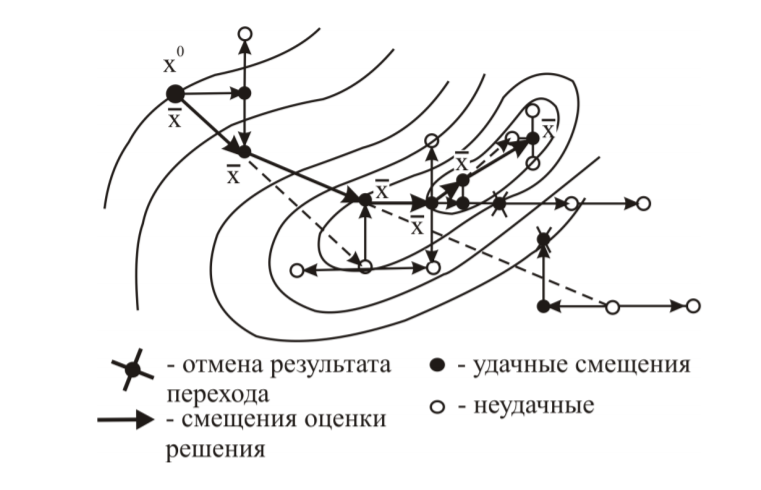
\includegraphics[width=1\linewidth]{figure/fig1.png}
			\caption{Пример итераций алгоритма Хука-Дживса} %% подпись к рисунку
			\label{fig:fig1}
		\end{minipage}
	\end{center}
\end{figure}	

\subsection{Decision tree}\label{SecDT}

Дерево принятия решений (decision tree) --- это средство, используемое для автоматического анализа больших массивов данных, который применяется в машинном обучении. Decision tree представляет собой бинарное дерево (дерево, в котором каждый не листовой узел имеет два дочерних узла). Его можно использовать как для решения задач классификации, так и для задач регрессии. При решении задач классификации каждый лист дерева помечается меткой класса, при этом несколько листьев могут иметь одну и ту же метку. В случае построения регрессии каждому листу дерева присваивается константа, поэтому получаемая функция аппроксимации является кусочно-постоянной.
В нашем случае decision tree строит функцию $\varphi(y)$ кусочно постоянную аппроксимацию$\varphi(y)$  в многомерном пространстве, обозначим как $z' = \psi(y)$ значение вычисленное по decision tree в точке $y$.

При реализации алгоритма  решения задач многомерной глобальной оптимизации с применением decision tree для выявления областей притяжения локальных минимумов нами были использованы алгоритмы из библиотеки OpenCV. OpenCV --- библиотека алгоритмов компьютерного зрения, обработки изображений и численных алгоритмов общего назначения с открытым кодом. Подробнее с decision tree можно ознакомиться в \cite{fio_bib16}


\section{Объединение локального метода оптимизации и GSA для решения многомерных задач}\label{SecGSAL}

В текущем разделе приведем подробное описание того, как мы использовали decision tree для выявления областей притяжения локальных экстремумов. 
В процессе работы GSA необходимо определить, стоит ли использовать текущую точку в качестве стартовой для локального метода или нет. Для этого можно проверить точки соседних испытаний и если среди них нет ни одной такой, значение функции в которой меньше, чем в текущей, то можно предположить, что мы находимся в области притяжения локального минимума. В этом случае из текущей точки можно запустить локальный метод, который быстро сойдется к локальному минимуму функции. 
Сделать это можно только в многомерном пространстве, а не на одномерном отрезке после редукции размерности.  
Во-первых, редуцированная функция $\varphi(y(x))$ меняет свои свойства: один локальный минимум в многомерном пространстве может разделиться на множество минимумов после редукции размерности. Во-вторых, после использования отображения $y(x)$ мы можем потерять информацию о взаимном расположении точек в исходном пространстве. Точки, расположенные близко в многомерном пространстве, могут оказаться существенно разнесенными на одномерном отрезке.


\begin{figure}[ht!]
	\begin{center}
		\begin{minipage}[h]{0.6\linewidth}
			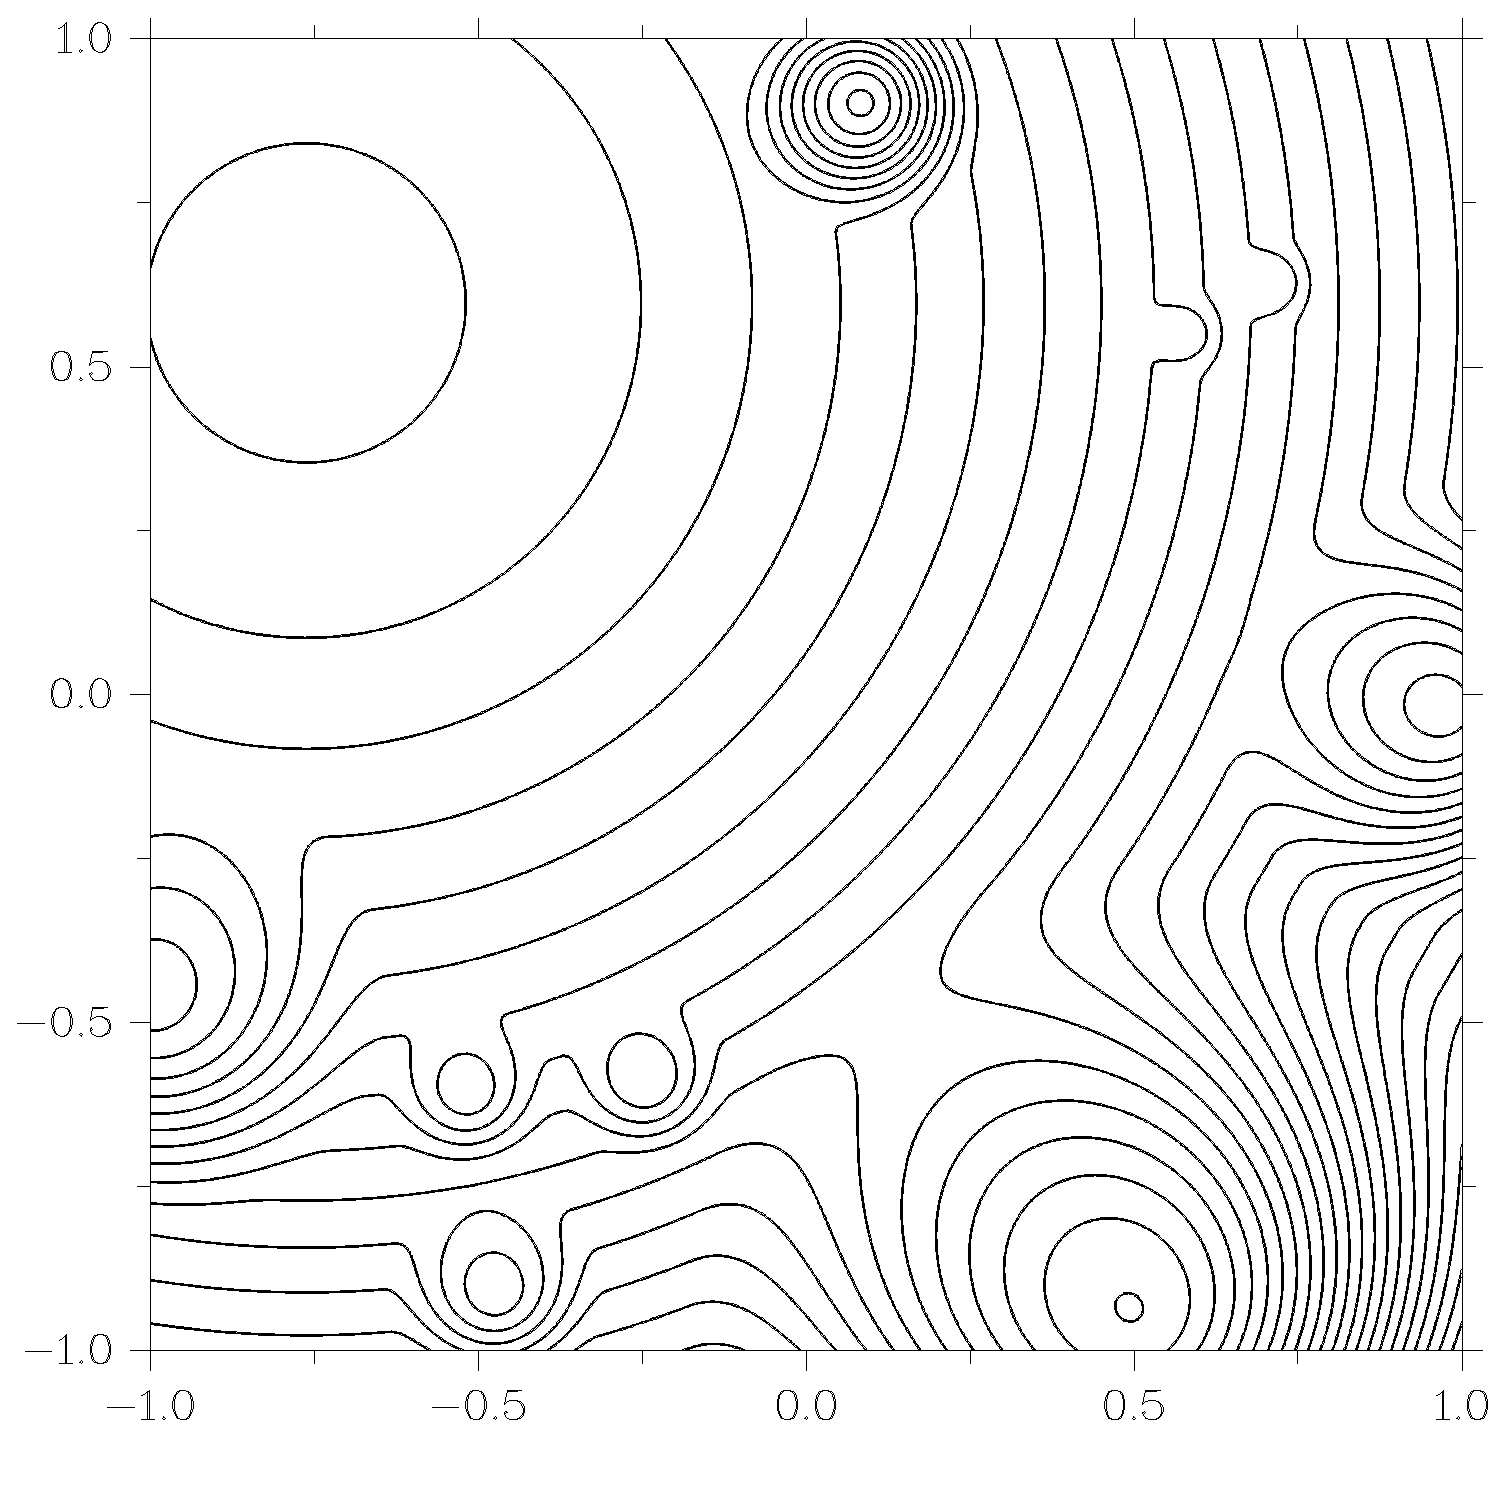
\includegraphics[width=1\linewidth]{figure/fig2.png}
			\caption{Функция из генератора gkls до использования кривых Пеано} %% подпись к рисунку
			\label{fig:fig2}
		\end{minipage}
	\end{center}
\end{figure}	

\begin{figure}[ht!]
	\begin{center}
		\begin{minipage}[h]{0.6\linewidth}
			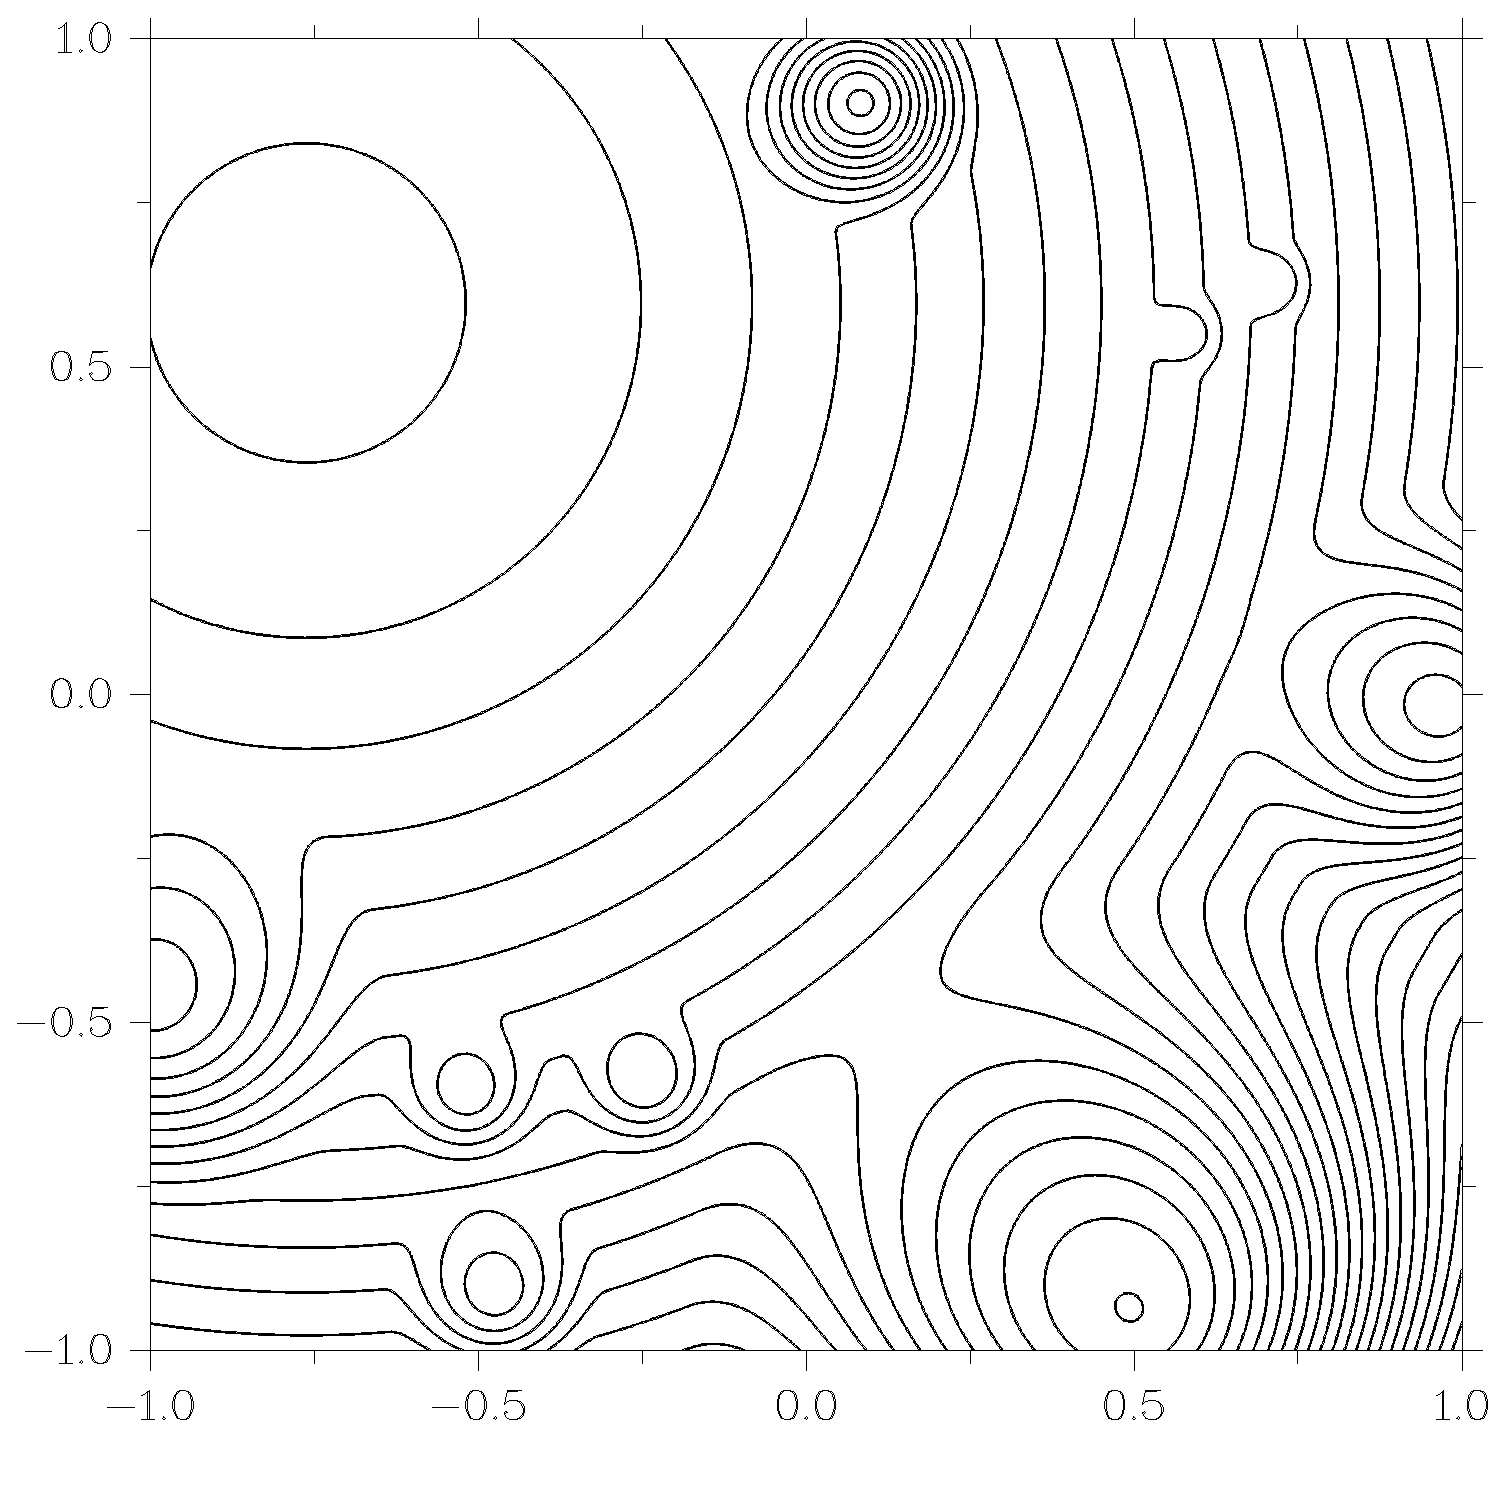
\includegraphics[width=1\linewidth]{figure/fig2.png}
			\caption{Рисунок с двумерным decision tree} %% подпись к рисунку
			\label{fig:fig2_2}
		\end{minipage}
	\end{center}
\end{figure}	




Поэтому определять области притяжения локальных экстремумов мы будем в исходном многомерном пространстве. Однако определить соседние точки в многомерном пространстве достаточно трудоемко, и для этого мы будем использовать decision tree. 

После проведения определенного числа trial (например, $100\ \ast\ N$), используем все накопившиеся точки для инициализации подходящей структуры данных и тренировки на ее основе decision tree. Чтобы проще было определить соседние точки, мы построим равномерную сетку с определенным шагом по каждой из координат, после чего вычислим значения аппроксимации целевой функции в этих точках с использованием дерева решений. Теперь, имея равномерную сетку точек и зная значение функции в каждой из них, найдем ближайшую, с точки зрения евклидова расстояния, к исходной. Эта ближайшая точка является проекцией исходной точки на равномерную сетку, на которой можно легко определить ее соседей. А так как decision tree строит аппроксимацию исходной функции (пусть и кусочно постоянную), то мы можем оценить значение функции в тех областях, в которых испытания ранее не проводились.

При рассмотрении соседей необходимо учитывать следующее: если хоть один из соседей имеет значение функции меньшее, чем в текущей точке, то запуск локального метода не нужен. Если хотя бы в одной из соседних точек значение функции такое же, как в текущей, то ее также необходимо проверить (т.е. найти всех ее соседей и проверять их аналогично). И только в том случае, если все значения функции в соседних точках больше, мы можем запускать локальный метод.

На Fig. \ref{fig:fig2} отображены линии уровня целевой функции с отображением точек испытаний, а на Fig. \ref{fig:fig2_2} отображено соответствующее decision tree. 

\section{Асинхронная схема распараллеливания алгоритма}\label{SecASP}

Способ организации параллельных вычислений, описанный в предыдущем разделе, подразумевает синхронное проведение $p$ поисковых испытаний в точках, вычисленных на текущей итерации. При этом переход к следующей итерации будет выполнен лишь после окончания проведения всех испытаний.
В случае различной трудоемкости проведения испытаний в разных точках области поиска данный подход может привести к дисбалансу вычислительной нагрузки. 
Исправить этот недостаток можно введением асинхронности.
Идея асинхронной схемы состоит в том, чтобы не дожидаться окончания проведения всех $p$ испытаний, а инициировать проведение нового испытания сразу же, как только было закончено хотя бы  одно их них. 

Предположим, что главный процесс вычисляет одну точку следующего trial на каждой итерации и отправляет ее рабочему процессу для выполнения trial. Отметим, что в прикладных оптимизационных задачах время выполнение trial рабочим процессом -- гораздо более затратная в вычислительном отношении операция, чем выбор мастером точки нового trial. Тем самым простой рабочих процессов будет пренебрежимо мал. В этом случае (в отличие от синхронных параллельных алгоритмов) общее количество trial, выполняемых каждым рабочим процессом, будет зависеть от вычислительных затрат на выполнение конкретного trial и не может быть оценено заранее. При описании параллельного алгоритма предположим, что в нашем распоряжении имеется $p+1$ вычислительных процессов: один главный и $p$ рабочих.

 В начале поиска главный процесс (допустим, это процесс с идентификатором $0$) инициирует параллельное выполнение $p$ trial в $p$ разных точках области поиска.

Две из этих точек являются граничными, а остальные -- внутренними, т.е. в точках $\{y\left(x^1\right),y\left(x^2\right),\ldots,y\left(x^p\right)\}$, где
$x^1=,x^p=,x^i\in\left(0,1\right),i=2,\ldots,p$.

Теперь предположим, что выполнено $k\geq0$ trial и рабочие процессы выполняют trial в точках $y\left(x^{k+1}\right),\;y\left(x^{k+2}\right),\ldots,\;y\left(x^{k+p}\right)$.

Каждый рабочий процесс, завершив в какой-то момент вычисление функции, отправляет главному процессу вычисленное значение. В свою очередь, главный процесс выбирает новую точку $x^{k+p+1}$ для рабочего процесса в соответствии с описанными ниже правилами. Заметим, что в этом случае мы будем иметь набор preimages of the trial points 
$I_k=\left\{x^{k+1},x^{k+2},\ldots,x^{k+p}\right\}$
в которых испытания уже начаты, но еще не завершены.

Таким образом параллельный асинхронный алгоритм глобальной оптимизации с использованием decision tree для выявления локальных областей состоит из следующих шагов:

\begin{enumerate}
\item  Упорядочить нижним индексом (в порядке возрастания) множество preimages of the trial points

\begin{displaymath}
X_k=\left\{x^1,x^2,\ldots,x^{k+p}\right\},
\end{displaymath}

содержащие все точки, в которых либо завершились, либо идут trial, т.е. получить упорядоченный набор

\begin{displaymath}
0=x_1<x_2<\ldots<x_{k+p}=1.
\end{displaymath}

\item  Вычислить значения

\begin{displaymath}
M_1=\max{\left\{\frac{\left|z_i-z_{i-1}\right|}{\left(x_i-x_{i-1}\right)^{1/N}}:x_{i-1}\notin I_k,x_i\notin I_k,2\le i\le k+p\right\}},
\end{displaymath}

\begin{displaymath}
M_2=\max{\left\{\frac{\left|z_{i+1}-z_{i-1}\right|}{\left(x_{i+1}-x_{i-1}\right)^{1/N}}:x_i\in I_k,2\le i<k+p\right\}},
\end{displaymath}

\begin{displaymath}
M=\max{\{}M_1,M_2\},
\end{displaymath}

где $ z_i=\varphi\left(y\left(x_i\right)\right)$, если $x_i\notin I_k,\;1\le i\le k+p$. Значения $z_i$ в точках $x_i\in I_k$ не определены, так как trial в точках $x_i\in I_k$ еще не завершены. Если значение $M$ равно $0$, то установить $M=1$.

\item  Сопоставить каждыму интервалу $\left(x_{i-1},x_i\right),\;x_{i-1}\notin I_k,x_i\notin I_k,\;2\le i\le k+p$ его характеристику $R\left(i\right)$, вычисляемую по формуле

\begin{displaymath}
R\left(i\right)=rM\Delta_i+\frac{\left(z_i-z_{i-1}\right)^2}{rM\Delta_i}-2\left(z_i+z_{i-1}\right),
\end{displaymath}

где $\Delta_i=\left(x_i-x_{i-1}\right)^{1/N}$ и $ r>1$ -- параметр надежности метода.

\item  Выбрать интервал $\left[x_{t-1},x_t\right]$, которому соответствует максимальная характеристика, т.е.

\begin{displaymath}
R\left(t\right)=\max{\left\{R\left(i\right):\;x_{i-1}\notin I_k,x_i\notin I_k,\;2\le i\le k+p\right\}}.
\end{displaymath}

\item  Определить новую точку испытания $y^{k+p+1}=y\left(x^{k+p+1}\right)$, прообразом которой является $x^{k+p+1}\in\left(x_{t-1},x_t\right)$, по формуле

\begin{displaymath}
x^{k+p+1}=\frac{x_t+x_{t-1}}{2}-\mathrm{sign}\left(z_t-z_{t-1}\right)\frac{1}{2r}\left[\frac{\left|z_t-z_{t-1}\right|}{M}\right]^N.
\end{displaymath}

\item  Получить вычисленное  значение функции с процесса $j$, добавить новый trial $z_j = f(y(x_j))$, к множеству $V$. 

%X_k=\left\{x^1,x^2,\ldots,x^{k+p}\right\}


\item 	Если $ k\ <\ 100\ast\ N$, то вернуться к шагу 1.

%\item 	Если используем decision tree не впервые, то перейти к пункту 15.

\item Создаем decision tree по множеству $I_k$, получаем функцию аппроксимации  $\psi(y)$.



\item 	Если используем decision tree впервые, то строим равномерную сетку

\begin{displaymath}
Y'=\{ y'\in\ R^N:\ a_i\le\  {y'_i}^k \le\ b_i,\ 1\le\ i\le\ N,\ 1\le k\le\ \sqrt[N]{300}  \}
\end{displaymath}

\item 	Вычисляем значения аппроксимации: $Z' = \{ z'=  \psi(y'), y' \in Y'\}$

\item Для всех точек $y'\in V$:

Находим точку $y'_q$ ближайшую  к $y'$,

Производим обход соседей $y'_q$ по описанному ранее принципу.

Если ни у одной соседней точки не нашлось значений функции меньших, чем в $y'_q$, то запускаем локальный метод.

Очищаем множество $V$.


\end{enumerate}

При вычислении точки очередного испытания главный процесс добавляет ее к множеству $I_k$ и отправляет рабочему процессу, который инициирует проведение испытания в ней.
Главный процесс завершает алгоритм, если выполняется одно из двух условий: $\Delta_t<$ или $k+p>K_{max}$.
Вещественное число $\epsilon>0$ и целое число $K_{max}>0$ являются параметрами алгоритма и соответствуют точности поиска решения и максимальному количеству испытаний соответственно.

\begin{figure}[ht!]

	\begin{center}
		\begin{minipage}[h]{0.9\linewidth}
			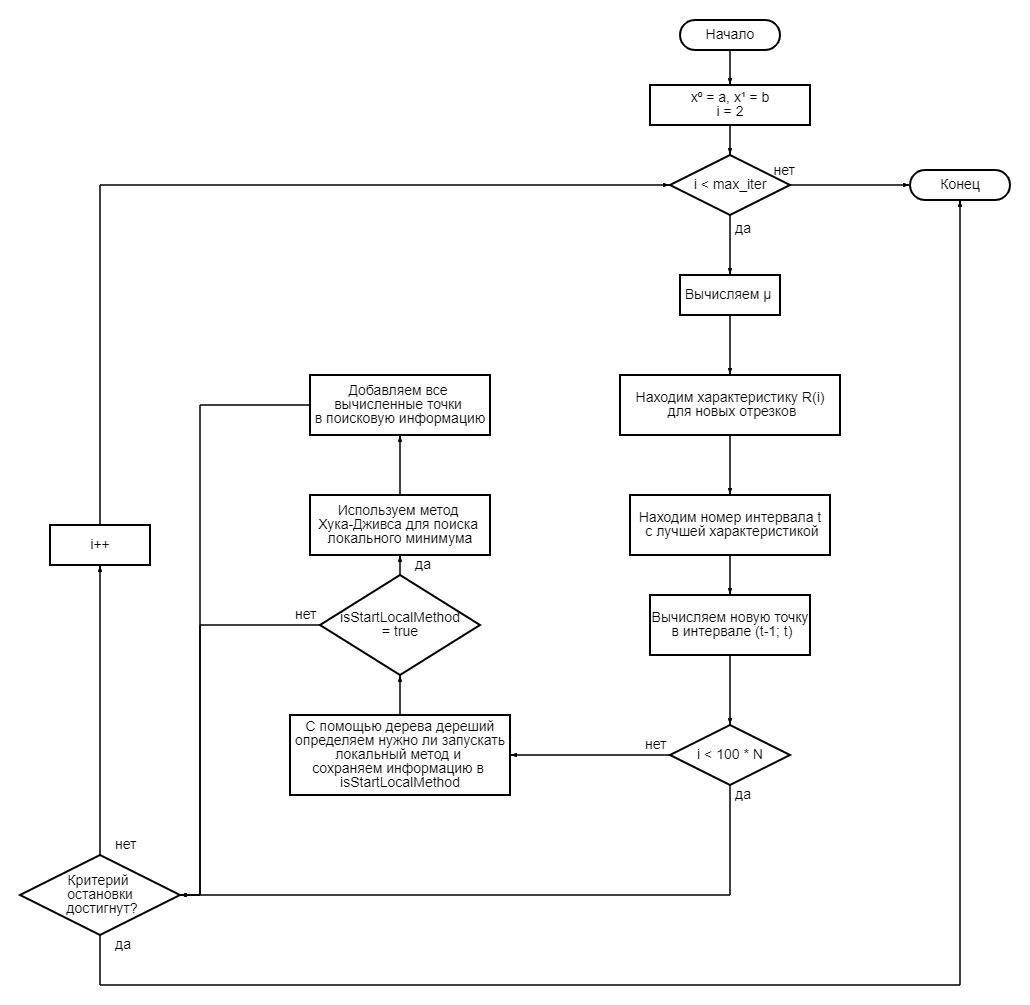
\includegraphics[width=1\linewidth]{figure/fig3.png}
			\caption{Блок-схема объединения АГП и метода Хука-Дживса с использованием decision tree} %% подпись к рисунку
			\label{fig:fig3}
		\end{minipage}
	\end{center}
\end{figure}


% переводить до этого раздела
\section{Результаты экспериментов}\label{SecR}


Вычислительные эксперименты были проведены на Lobachevsky supercomputer. Один узел кластера состоит из двух процессоров Intel Sandy Bridge E5-2660 2.2 GHz, 64 Gb RAM. 

\cite{fio_bib13, fio_bib17} описывает генераторы GKLS, которые могут генерировать многоэкстремальные задачи оптимизации с известными свойствами: глобальным минимумом и его значением, количеством локальных минимумов и так далее.

В таблице \ref{tab:1} приведено среднее количество итераций методов глобальной оптимизации при решении серии задач из генератора GKLS. Знак «>» указывает на ситуацию, когда не все задачи были решены, в скобках указано количество нерешенных задач. Как видно, АГП превосходит методы DIRECT и DIRECTl по среднему числу итераций. 




\begin{table}[!ht]
    \caption{Среднее число итераций}
    \label{tab:1}
    \centering
    \begin{tabular}{|l|l|l|l|l|}
    \hline
        N & Problem class & DIRECT & DIRECTl & АГП  \\ \hline
        4 & Simple & >47282 (4) & 18983 & 11953  \\ \hline
        ~ & Hard & >95708 (7) & 68754 & 25263  \\ \hline
        5 & Simple & >16057 (1) & 16758 & 15920  \\ \hline
        ~ & Hard & >217215 (16) & >269064 (4) & >148342 (4)  \\ \hline
    \end{tabular}
\end{table}




Ниже приведены результаты сравнения двух алгоритмов – асинхронного АГП и его объединение с локальным методом (методом Хука-Дживса) при использовании decision tree. Численное сравнение проводилось на классах функций Simple и Hard размерности 2, 3, 4 и 5 из \cite{fio_bib19}. Критерием остановки служило попадание trial в эпсилон окрестность истинного глобального минимума. 

В таблице \ref{tab:2} представлено среднее количество итераций, и ускорение по времени относительно последовательного запуска. Распараллеливание  осуществлялось с применением асинхронного MPI алгоритма. При этом, запуск производился на 4 процессах, а следовательно, на каждой итерации вычислялось 3 точки. Значение в скобках (если оно есть) показывает количество не решенных задач. Это означает, что было достигнут максимум по числу проводимых итераций, но в окрестность глобального минимума точка так и не попала.


В таблице \ref{tab:2} приведены результаты сравнения двух алгоритмов –-- асинхронного алгоритма глобального поиска (АГП) и АГП с использованием деревьев решений для выявления областей притяжения локальных минимумов (Деревья решений). Численное сравнение проводилось на классах функций Simple и Hard размерности 2, 3, 4 и 5 из \cite{fio_bib19}. Алгоритм прекращал свою работу как только поражалась точка испытания в эпсилон окрестность истинного глобального минимума. В таблице сравнивается среднее количество итераций, и ускорение по времени относительно последовательного запуска. Распараллеливание  осуществлялось с применением асинхронного MPI алгоритма. При этом, запуск производился на 8 процессах, а следовательно, на каждой итерации вычислялось 7 точек.


\begin{table}[h!]
	\caption{Среднее число итераций и среднее число trial, проводимое разными алгоритмами}
	\label{tab:2}
	\centering
	\begin{tabular}{|c|c|c|c|c|c|}
		\hline
		
		N & Класс задачи & \multicolumn{2}{c|}{Среднее число итераций} & \multicolumn{2}{c|}{Ускорение} \\ \hline
		& ~ & АГПА & decision tree & АГПА & decision tree \\ \hline
		& Simple & 3823,1   & 485,6  & 7,4   & 84,1 \\ \hline
		2  & Hard & 787,6    & 304,2  & 13,8  & 62,4  \\ \hline
		& Simple & 5700,5   & 720,1  & 5,6   & 63,6  \\ \hline
		3  & Hard & 2411,9   & 634,3  & 5,0   & 29,8  \\ \hline
		& Simple & 31101,5  & 1037,4 & 5,1   & 200,7  \\ \hline
		4  & Hard & 10418,1  & 816,2  & 6,9   & 122,7  \\ \hline
		& Simple & 163313,5 & 1204,2 & 4,8   & 781,9  \\ \hline
		5  & Hard & 27524,5  & 999,4  & 4,6   & 161,5  \\ \hline
	\end{tabular}
\end{table}

Как видно из таблицы ускорение по числу итераций достаточно велико, причем на задачах любой размерности. 

\section{Заключение}\label{SecC}

Методы глобальной оптимизации являются областью активных научных исследований.  В результате работы удалось успешно объединить алгоритм глобального поиска вместе с поиском локального минимума методом Хука-Дживса. С целью экспериментального подтверждения теоретических свойств рассматриваемого алгоритма были так же проведены вычислительные эксперименты на серии из сотни тестовых задач. 

При использовании в качестве определяющего правила о необходимости запуска локального метода decision tree, нам удалось получить достаточно хорошее ускорение. Применяя параллельную версию Алгоритма Глобального поиска ускорение удалось сохранить, что является несомненным преимуществом. Таким образом, наша схема позволяет получить преимущество от обоих из подходов (и от распараллеливания, и от запуска локального метода).





%
% ---- Bibliography ----
%
\bibliographystyle{spmpsci}
\begin{thebibliography}{6}
%

\bibitem{fio_bib1}
Ferreiro A.M., Garcia J.A., Lopez-Salas J.G., Vazquez C. An efficient implementation of parallel simulated annealing algorithm in GPUs // Journal of global optimization. — 2013. — Vol. 57, No. 3. — P. 863–890.

\bibitem{fio_bib2}
Garcia-Martinez J.M., Garzon E.M., Ortigosa P.M. A GPU implementation of a hybrid evolutionary algorithm: GPuEGO // Journal of super-computing. — 2014. — Vol. 70, No. 2. — P. 684–695.

\bibitem{fio_bib3}
Langdon W.B. Graphics processing units and genetic programming: an overview // Soft Computing. — 2011. — Vol. 15, No 8. — P. 1657–1669.

\bibitem{fio_bib4}
Евтушенко Ю.Г., Малкова В.У., Станевичюс А.А. Параллельный поиск глобального экстремума функций многих переменных // Ж. вычисл. матем. и матем. физ. — 2009. — Т. 49, №2. — С. 255–269.

\bibitem{fio_bib5}
He J., Verstak A., Watson L.T., Sosonkina M. Design and implementation of a mas-sively parallel version of DIRECT // Computational optimization and applications. — 2008. — Vol. 40, No. 2. — P. 217–245

\bibitem{fio_bib6}
Paulavicius R., Žilinskas J., Grothey A. Parallel branch and bound for global optimiza-tion with combination of Lipschitz bounds // Optimization methods and software. — 2011. — Vol. 26, No. 3. — P. 487–498.

\bibitem{fio_bib7}
Глобальная оптимизация: приложения и вычислительная сложность. %URL: http://hpc-education.unn.ru/ru/globopt/глобальная-оптимизация-приложения-и (дата обращения: 10.10.2020).

\bibitem{fio_bib8}
Захарова Е.М., Минашина И.К. Обзор методов многомерной оптимизации. Информационные процессы // том 14 - №3 – 2014 - С. 256-274.

\bibitem{fio_bib9}
Городецкий С. Ю. Методические материалы к лабораторной работе «Вычислительные методы поиска локальных минимумов функций», 2001.% URL: http://itmm.unn.ru/files/2016/09/MO_Lab2_LocOpt.pdf (дата обращения: 09.07.2022).

\bibitem{fio_bib10}
Шефов К. С., Степанова М. М. Реализация и применение параллельного алгоритма глобального поиска минимума к задаче оптимизации параметров молекулярно-динамического потенциала ReaxFF: %URL: http://crm.ics.org.ru/uploads/crmissues/crm_2015_3/15750.pdf, 2015 (дата обращения: 13.10.2020).

\bibitem{fio_bib11}
Gergel V.P. A global optimization algorithm for multivariate functions with lipschitzian first derivatives / Gergel V.P. // Journal of Global Optimization. – 1997. – Vol. 10, No. 3. – P. 257-281.

\bibitem{fio_bib12}
Barkalov K.A. A global optimization technique with an adaptive order of checking for constraints / Barkalov K.A., Strongin R.G. // Computational Mathematics and Mathematical Physics. – 2002. – Vol. 42, No. 9. – P. 1289-1300.

\bibitem{fio_bib13}
Gaviano, M. Software for generation of classes of test functions with known local and global minima for global optimization/ M. Gaviano, D. Lera, D. E. Kvasov, Y. D. Sergeyev // ACM Transactions on Mathematical Software. – 2003. – Vol. 29. – P. 469-480.

\bibitem{fio_bib14}
Химмельблау Д. Прикладное нелинейное программирование // М.: Мир - 1975 - 536 с. 

\bibitem{fio_bib15}
Nelder J., Mead R. A simplex method for function minimization // Computer Journal - 7(4) – 1965 - P. 308-313.

\bibitem{fio_bib16}
OpenCV (Open Source Computer Vision) documentation. %URL: https://docs.opencv.org/4.x/dc/dd6/ml_intro.html (дата обращения: 10.07.2022)

\bibitem{fio_bib17}
Сергеев, Я.Д. Диагональные методы глобальной оптимизации / Я.Д. Сергеев, Д.Е. Квасов – М.: Физматлит, 2008. – 352 c.

\bibitem{fio_bib18}
Sysoyev, A.,  Barkalov, K.,  Sovrasov, V.,  Lebedev, I.,  Gergel, V. Globalizer – A parallel software system for solving global optimization problems. Lecture Notes in Computer Science. Volume 10421 LNCS, 2017, Pages 492-499

\bibitem{fio_bib19}
Sergeyev, Ya.D. Global search based on efficient diagonal partitions and a set of Lipschitz constants / Ya.D. Sergeyev, D.E. Kvasov // SIAM Journal on Optimization. – 2006. Vol. 16, No. 3. – P. 910–937

\bibitem{fio_bib20}
Стронгин Р.Г. Параллельные вычисления в задачах глобальной оптимизации / Стронгин Р.Г., Гергель В.П., Гришагин В.А., Баркалов К.А. – М.: Издательство Московского университета, 2013. 280 с.









\end{thebibliography}
\end{document}
